\begin{center}
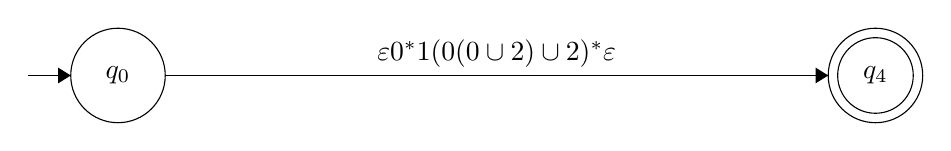
\begin{tikzpicture}[scale=0.2]
\tikzstyle{every node}+=[inner sep=0pt]
\draw [black] (16.5,-17.2) circle (3);
\draw (16.5,-17.2) node {$q_0$};
\draw [black] (64.6,-17.2) circle (3);
\draw (64.6,-17.2) node {$q_4$};
\draw [black] (64.6,-17.2) circle (2.4);
\draw [black] (10.8,-17.2) -- (13.5,-17.2);
\fill [black] (13.5,-17.2) -- (12.7,-16.7) -- (12.7,-17.7);
\draw [black] (19.5,-17.2) -- (61.6,-17.2);
\fill [black] (61.6,-17.2) -- (60.8,-16.7) -- (60.8,-17.7);
	\draw (40.55,-16.7) node [above] {$\varepsilon0^*1(0(0\cup2)\cup2)^*\varepsilon$};
\end{tikzpicture}
\end{center}
